\documentclass[11pt]{article}

% ---------------------------------------------------------------------------
% Packages
% ---------------------------------------------------------------------------
\usepackage[utf8]{inputenc}
\usepackage[T1]{fontenc}
\usepackage[a4paper,margin=1in]{geometry}
\usepackage{microtype}
\usepackage{xcolor}
\usepackage{booktabs}
\usepackage{tabularx}
\usepackage{array}
\usepackage{enumitem}
\usepackage{caption}
\usepackage{adjustbox}
\usepackage{float}
\usepackage{tikz}
\usetikzlibrary{positioning,arrows.meta,shapes.geometric,fit,backgrounds,calc}
\usepackage[colorlinks=true,linkcolor=black,urlcolor=blue]{hyperref}

% ---------------------------------------------------------------------------
% Palette (blue = user-authored, grey = SDK-owned, white = engine/registry)
% ---------------------------------------------------------------------------
\definecolor{userblue}{HTML}{E8F0FE}
\definecolor{userstroke}{HTML}{3B78E7}
\definecolor{sdkgrey}{HTML}{ECEEF1}
\definecolor{sdkstroke}{HTML}{8A9099}
\definecolor{engwhite}{HTML}{FFFFFF}
\definecolor{subgbg}{HTML}{FAFBFD}
\definecolor{codebg}{HTML}{F4F4F6}

% ---------------------------------------------------------------------------
% Shared node / edge styles
% ---------------------------------------------------------------------------
\tikzset{
  box/.style   = {rounded corners=3pt, draw, align=center, font=\small,
                  inner sep=5pt, minimum height=11mm, minimum width=30mm,
                  line width=0.6pt},
  user/.style  = {box, fill=userblue, draw=userstroke},
  sdk/.style   = {box, fill=sdkgrey,  draw=sdkstroke},
  eng/.style   = {box, fill=engwhite, draw=sdkstroke, line width=0.9pt},
  pill/.style  = {box, minimum width=40mm, minimum height=18mm, fill=engwhite,
                  draw=sdkstroke, line width=1pt},
  grp/.style   = {rounded corners=6pt, draw=sdkstroke, dashed, fill=subgbg,
                  inner sep=10pt},
  arr/.style   = {-{Stealth[length=2.6mm]}, semithick, draw=sdkstroke},
  arrf/.style  = {arr, dashed},
  arrd/.style  = {-{Stealth[length=2.4mm]}, line width=0.8pt, dotted, draw=userstroke},
  lab/.style   = {font=\scriptsize, fill=white, inner sep=1.5pt, midway},
  alab/.style  = {font=\scriptsize\itshape, text=userstroke, fill=white, inner sep=1.5pt, midway},
  agent/.style = {box, fill=userblue, draw=userstroke, dotted, line width=1pt, font=\small\itshape},
}

\newcommand{\code}[1]{\texttt{\small #1}}
\newcommand{\note}[1]{%
  \par\vspace{2pt}%
  \noindent\colorbox{codebg}{%
    \begin{minipage}{0.965\linewidth}\small\itshape #1\end{minipage}}%
  \par\vspace{4pt}}

\captionsetup{font=small,labelfont=bf,width=0.92\linewidth}
\setlist[itemize]{leftmargin=1.4em, itemsep=2pt, topsep=3pt}
\renewcommand{\arraystretch}{1.25}

% ---------------------------------------------------------------------------
\title{\textbf{EvSys --- Turn your coding agents into a continual-learning lab}}
\author{}
\date{}

\begin{document}
\maketitle
\vspace{-3.2em}

\begin{center}
\begin{minipage}{0.9\linewidth}\itshape\small
Infrastructure for thousands of task-specialised models that learn continuously
from every interaction.
\end{minipage}
\end{center}

\vspace{0.8em}
\hrule
\vspace{1.4em}

% ===========================================================================
\section{Enabling a continual learning system}
% ===========================================================================
We believe the future of AI is not a handful of giant generalist models, but
\textbf{thousands of task-specialised models that learn continuously from every
interaction}. In that future, \textbf{enterprises will build a continual-learning
system for every use-case} they have --- each one a model that keeps getting
better at its specific job. Realising that future requires a new layer of
infrastructure: the
\textbf{autoresearch} infrastructure for continuously learning models --- the
abstractions that let a system discover what to learn, train on it, and ship it
autonomously and safely. \textbf{The SDK builds that layer.} The SDK abstracts away all the complexities related to training models and makes coding agents and you focus only on two parts - \textbf{data} and the \textbf{algorithm}

To make that autoresearch work, you need to both \textbf{standardise} and
\textbf{centralise} the entire history of experiments, so that coding agents
have the context they need. That is what this SDK does: it lets coding agents
--- and you --- focus on the training experiments themselves (finding the right
\textbf{data} and \textbf{recipe}), while the SDK handles the standardisation,
the centralisation, and the supply of the right context to you and your coding
agents. Without this standardisation a coding agent just sees a pile of ad-hoc
training scripts: every experiment looks different, so it cannot reason across
them or build on what worked. Standardisation is what makes the history of
experiments legible enough for an agent to learn from.

The end state is a closed loop. A deployed model produces \textbf{production
traces}; a lightweight \textbf{agent decides} whether a given trace is worth
learning from and, if so, triggers \textbf{autoresearch}; the autoresearch loop
runs a series of educated experiments and trains a candidate checkpoint;
\textbf{deployment evals} then judge whether that checkpoint is genuinely better
than what is in production --- and only then is it \textbf{deployed}. The freshly
deployed model produces new traces, and the loop continues, so the system
improves with every interaction. What we release today is \textbf{Phase 1}: the
autoresearch loop --- everything the rest of this document describes.

\begin{figure}[h]
\centering
\begin{adjustbox}{max width=\linewidth}
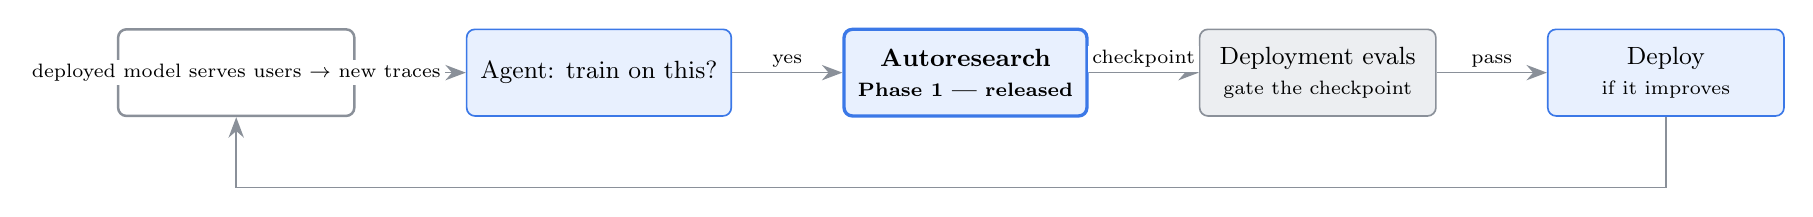
\begin{tikzpicture}[node distance=10mm and 14mm]
  \node[eng] (prod) {Production traces};
  \node[user, right=of prod] (decide) {Agent: train on this?};
  \node[eng, right=of decide, line width=1.2pt, draw=userstroke, fill=userblue]
        (auto) {\textbf{Autoresearch}\\\scriptsize \textbf{Phase 1 --- released}};
  \node[sdk, right=of auto] (deval) {Deployment evals\\\scriptsize gate the checkpoint};
  \node[user, right=of deval] (deploy) {Deploy\\\scriptsize if it improves};

  \draw[arr] (prod)   -- (decide);
  \draw[arr] (decide) -- node[lab,above]{yes} (auto);
  \draw[arr] (auto)   -- node[lab,above]{checkpoint} (deval);
  \draw[arr] (deval)  -- node[lab,above]{pass} (deploy);
  \draw[arr] (deploy.south) -- ++(0,-9mm) -| (prod.south);
  \node[lab] at ($(prod)!0.5!(deploy) + (0,-12mm)$)
        {deployed model serves users $\to$ new traces};
\end{tikzpicture}
\end{adjustbox}
\caption{The continual-learning system. A deployed model produces traces; an
agent decides whether to learn from them and triggers \textbf{autoresearch}
(this SDK), which trains a candidate checkpoint; deployment evals gate whether it
ships. The blue \textbf{autoresearch} stage --- and only that stage --- is what we
release as Phase 1.}
\end{figure}

\subsection{Why two agents, and why autoresearch?}
The design rests on a deliberate split of work across \textbf{two agents}.

The \textbf{first agent is a light, fast decision-maker}. It watches incoming
production traces and decides whether a batch is worth learning from. Because it
gates the expensive step, it must be cheap and quick --- and it needs \emph{no}
context of previous experiments. If it says yes, it hands off to the second
stage, where the real budget is spent.

\textbf{That second stage is autoresearch} --- a heavier, budgeted search for the
right training recipe. We frame continual learning as autoresearch on purpose:
there is \textbf{no single algorithm} that enables continual learning across all
data; different data demands different recipes. So a capable agent must
autonomously run experiments, recover from training collapses, and decide which
checkpoint is finally worth deploying. That is exactly what the autoresearch loop
does --- which is why training a model with this SDK is, by construction, a
building block of the larger continual-learning system.

% ===========================================================================
\section{Why do we need it?}
% ===========================================================================
We believe in a world where there will be thousands of custom models, each
specialised for a particular task. Training a model that sits on the Pareto
frontier of the accuracy-versus-cost curve is a cumbersome task: it comes down
to deciding what data goes into training and which recipe is used. We believe
auto-research is the answer to this problem: coding agents run a series of
educated experiments and finally train a model that meets the targeted
requirements.

Tinker-protocol-compatible training infrastructure is increasingly making it
easy to train models, abstracting away the model infrastructure and the
complexities of training large models. However, engineers and researchers still
have to focus on a lot of plumbing code and experiment management. With this
SDK, launching an experiment is now as simple as writing a YAML file.
% TODO : keep this as secondary point

% ===========================================================================
\section{Design principles}
% ===========================================================================

\begin{itemize}
  \item \textbf{Separate data from recipe.} We believe that to train a frontier
    model you need to choose two main things: the \textbf{data} and the
    \textbf{training recipe}. All of our abstractions are built around this, with
    a clear separation between the two. It lets you edit and run experiments
    across different training data and algorithms, while abstracting away all the
    plumbing around each experiment.
  \item \textbf{Any algorithm or data ablation.} The
    abstractions are general enough to express any training algorithm and any
    data ablation, and every run is scored against a benchmark, so each variation
    you try is linked directly to downstream task performance.
  \item \textbf{Capture context for auto-research.} To enable auto-research, you
    need to provide the right context to your coding agents. Our main class is
    the \code{Experiment} class: for every experiment you can store a hypothesis
    (the reason for running it) and a conclusion (its result).

    \item \textbf{Single line experiment configs enables auditability} Launch experiments with a single-line, the SDK handles all the management. 
    
  \item \textbf{Built for multi-turn, agentic workloads.} Workloads are moving
    from single-turn chatbots to more agentic, multi-turn workflows. We therefore
    support multi-turn reinforcement learning inside custom agent harnesses, so
    you can run ablations on both the algorithm and the harness together.
  \item \textbf{Standardise without losing flexibility.} When a coding agent
    gathers context across hundreds of experiments, standardisation helps a lot
    with understanding each one. For this reason we have chosen highly
    customisable yet general data models, giving you flexibility while keeping
    the experiments standardised.

    
\end{itemize}

% ===========================================================================
\section{The three pillars at a glance}
% ===========================================================================

A single \code{ExperimentConfig} (one YAML file) drives one run. Conceptually
the run is a left-to-right pipeline: the \textbf{Data} surface produces typed
rows, the \textbf{Training} surface consumes them and emits checkpoints, and the
\textbf{Evaluation} surface scores those checkpoints, with validation looping
back to steer model selection.

\begin{figure}[h]
\centering
\begin{adjustbox}{max width=\linewidth}
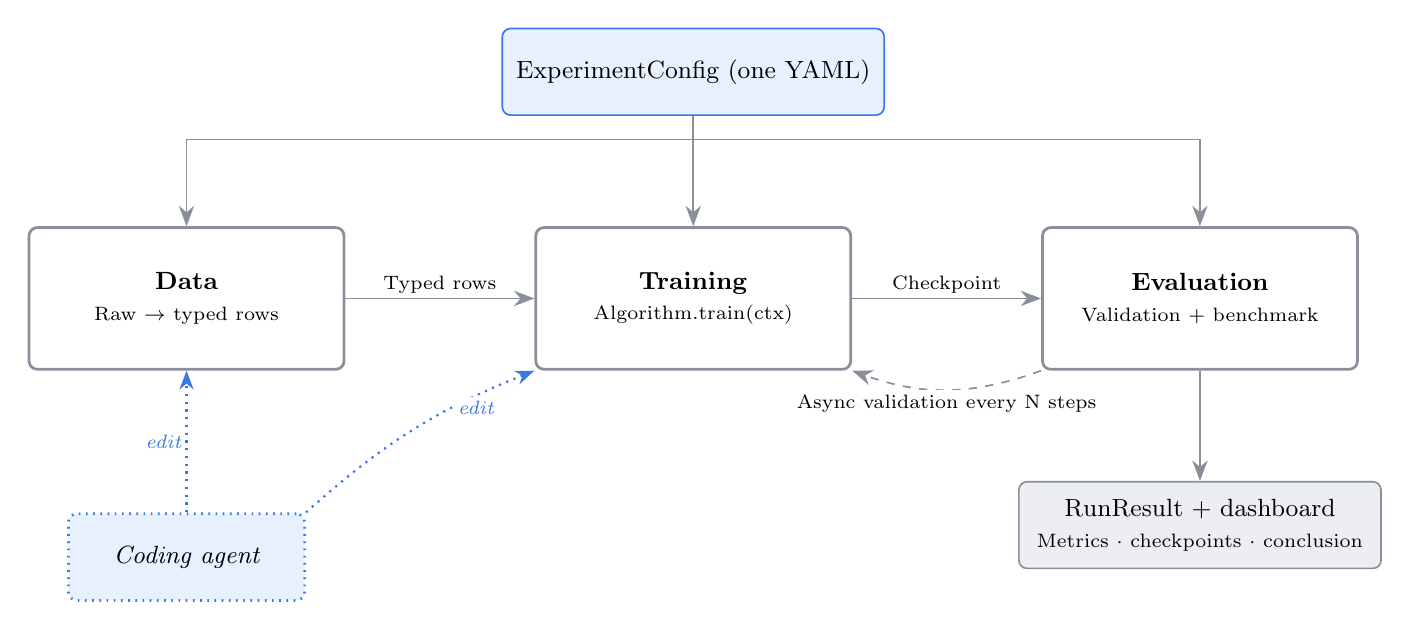
\begin{tikzpicture}[node distance=24mm]
  \node[pill] (data)  {\textbf{Data}\\\scriptsize Raw $\to$ typed rows};
  \node[pill, right=of data]  (train) {\textbf{Training}\\\scriptsize Algorithm.train(ctx)};
  \node[pill, right=of train] (eval)  {\textbf{Evaluation}\\\scriptsize Validation + benchmark};

  \node[user, above=14mm of train] (cfg) {ExperimentConfig (one YAML)};
  \node[sdk,  below=14mm of eval, minimum width=46mm] (out)
        {RunResult + dashboard\\\scriptsize Metrics $\cdot$ checkpoints $\cdot$ conclusion};

  \draw[arr] (cfg.south) -- ++(0,-3mm) -| (data.north);
  \draw[arr] (cfg.south) -- (train.north);
  \draw[arr] (cfg.south) -- ++(0,-3mm) -| (eval.north);

  \draw[arr] (data)  -- node[lab,above]{Typed rows} (train);
  \draw[arr] (train) -- node[lab,above]{Checkpoint} (eval);
  \draw[arr] (eval.south) -- (out.north);

  \draw[arrf] (eval.south west) to[bend left=20]
        node[lab,below]{Async validation every N steps} (train.south east);

  % --- coding agent acts on the Data + Training surfaces ---
  \node[agent, below=18mm of data] (cagent) {Coding agent};
  \draw[arrd] (cagent.north) -- node[alab,left]{edit} (data.south);
  \draw[arrd] (cagent.north east) to[bend left=10]
        node[alab,below,pos=0.78]{edit} (train.south west);
\end{tikzpicture}
\end{adjustbox}
\caption{Top-level dataflow. The user authors one config (blue); the SDK (grey)
runs Data $\to$ Training $\to$ Evaluation and records a RunResult. Evaluation's
in-loop validation feeds back into training to drive model selection, while the
benchmark is scored once at the end. The dotted arrows mark the two extension
points a \textbf{coding agent} can author: a \code{transforms()} on the data
surface, and a \code{StepBuilder} on the training surface.}
\end{figure}

% ===========================================================================
\section{The Experiment}
% ===========================================================================

Everything in the SDK is organised around the \textbf{Experiment}, the unit
of scientific work. An experiment is two things together: an \textbf{experiment
config} (a single YAML file that declares the data, the recipe, and how to
evaluate) and a short \textbf{SDK script} that launches it. That is all it takes
to run.

Because an experiment is a scientific act, it carries its reasoning with it.
Every experiment records a \textbf{hypothesis} (the reason you are running
it) and, once finished, a \textbf{conclusion} (what you learned). This is
what keeps the history legible: a coding agent (or a teammate) reading back over
hundreds of past experiments sees not just numbers, but the question each one
asked and the answer it reached.

One experiment need not be a single run. From the same config you can fan out
into many \textbf{runs} (a sweep over learning rates, datasets, or
algorithms) and repeat each across several seeds to measure variance. The SDK
runs them all, scores each against your chosen \textbf{success metric}, and
selects the best to form the experiment's conclusion. You describe the
variations declaratively; the SDK handles the orchestration, the dashboard, and
the comparison.

Each run is where the two choices come together: a choice of \textbf{data} and a
choice of \textbf{recipe} (the training algorithm and how it is evaluated). The
rest of this document walks through those two surfaces in turn: first how the
data is shaped, then how training and evaluation run.

% ===========================================================================
\section{Data surface}
% ===========================================================================

Standardize \emph{anything} into a few typed shapes, then hand those to the
algorithm. Loading, caching, and conversion are the SDK's job; the user only
declares a source and (optionally) custom transforms.

The raw data is a \code{jsonl} file. A \textbf{transform} is the piece a coding
agent writes to convert that raw data into one of the typed formats
(\code{ChatMessagesRow} / \code{PromptExample} / \code{HarborTask}), which is
then consumed by the training loop ahead. This separation is what lets you run
\textbf{data experiments}: the same raw data, but different \emph{actual}
training data depending on the transform (for example, thinking
vs.\ non-thinking traces, with or without system prompts, or different
templating) without ever touching the source.

\begin{figure}[H]
\centering
\begin{adjustbox}{max width=\linewidth}
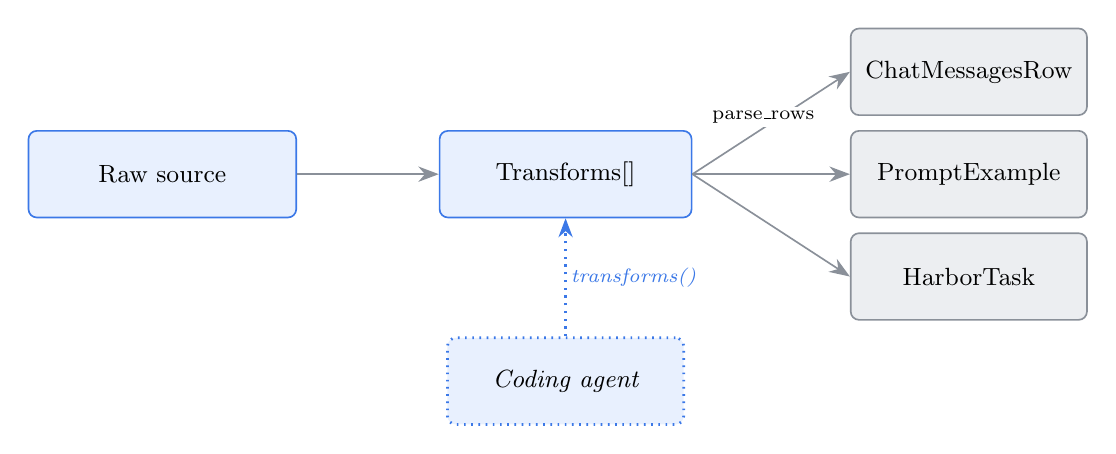
\begin{tikzpicture}[node distance=18mm]
  \node[user, minimum width=34mm] (src) {Raw source};
  \node[user, right=of src, minimum width=32mm] (tf) {Transforms[]};

  \node[sdk, right=20mm of tf, yshift=13mm]  (cm) {ChatMessagesRow};
  \node[sdk, right=20mm of tf]               (pe) {PromptExample};
  \node[sdk, right=20mm of tf, yshift=-13mm] (ht) {HarborTask};

  \draw[arr] (src) -- (tf);
  \draw[arr] (tf.east) -- node[lab,above,pos=0.45]{parse\_rows} (cm.west);
  \draw[arr] (tf.east) -- (pe.west);
  \draw[arr] (tf.east) -- (ht.west);

  % --- coding agent authors the transform ---
  \node[agent, below=15mm of tf] (cagent) {Coding agent};
  \draw[arrd] (cagent.north) -- node[alab,right]{transforms()} (tf.south);
\end{tikzpicture}
\end{adjustbox}
\caption{Data pipeline. A declared source is passed through ordered
\code{Transform}s and converted (\code{parse\_rows}) into one of three typed
shapes. The shape chosen depends on the algorithm: chat SFT consumes
\code{ChatMessagesRow}, SDFT consumes \code{PromptExample}, RL consumes
\code{HarborTask}.}
\end{figure}



% ===========================================================================
\section{Training \& Evaluation}
% ===========================================================================

You focus on the \textbf{algorithm}; the SDK does the plumbing. To define a new
training method you implement a single function, \code{build\_batch}. This
function is the algorithm: it does the math for one optimisation step and returns
both the batch of data and the \textbf{loss function} to apply to it, which the
training loop then uses to update the model. Everything around it is handled for
you: allocating the backend, the forward/backward and optimiser steps, batching,
checkpointing, and running validation every N steps. A reference algorithm is
only a few dozen lines.

\begin{figure}[H]
\centering
\begin{adjustbox}{max width=\linewidth}
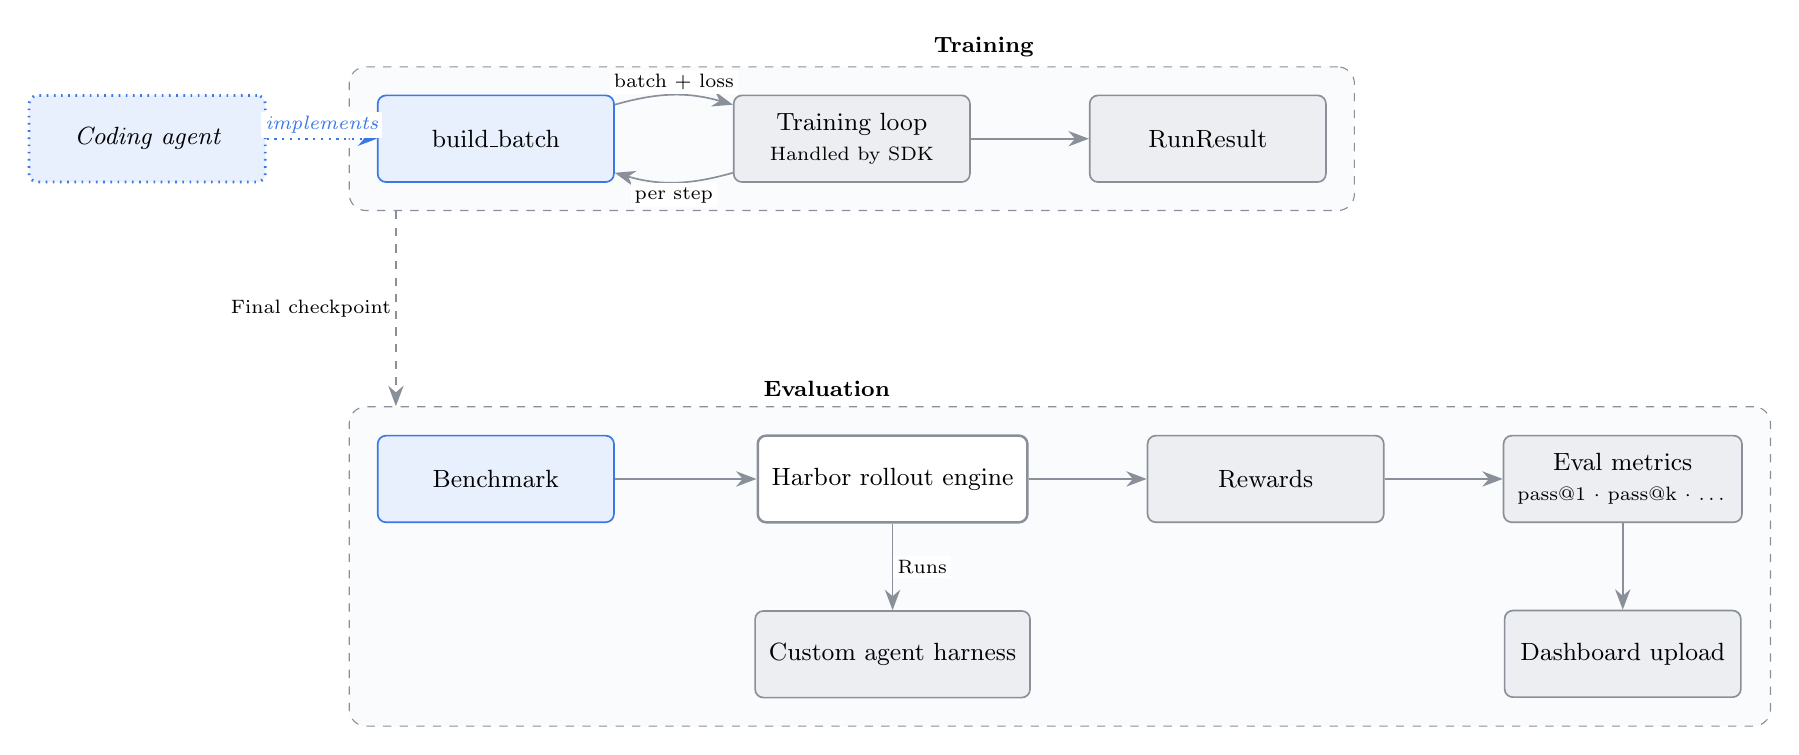
\begin{tikzpicture}[node distance=9mm and 15mm]
  % ---------------- Training lane ----------------
  \node[user] (bb)   {build\_batch};
  \node[sdk,  right=of bb]   (loop) {Training loop\\\scriptsize Handled by SDK};
  \node[sdk,  right=of loop] (rr)   {RunResult};
  \node[agent, left=14mm of bb] (cagent) {Coding agent};
  \draw[arr] (bb) to[bend left=16] node[lab,above]{batch + loss} (loop);
  \draw[arr] (loop) to[bend left=16] node[lab,below]{per step} (bb);
  \draw[arr] (loop)--(rr);
  \draw[arrd] (cagent.east) -- node[alab,above]{implements} (bb.west);
  \begin{scope}[on background layer]
    \node[grp, fit=(bb)(loop)(rr),
      label={[font=\footnotesize\bfseries]above right:{Training}}] (tlane){};
  \end{scope}

  % ---------------- Evaluation lane ----------------
  \node[user, below=32mm of bb] (bmk) {Benchmark};
  \node[eng,  right=18mm of bmk] (engn) {Harbor rollout engine};
  \node[sdk,  below=11mm of engn] (harn) {Custom agent harness};
  \node[sdk,  right=of engn] (rew) {Rewards};
  \node[sdk,  right=of rew]  (met) {Eval metrics\\\scriptsize pass@1 $\cdot$ pass@k $\cdot$ \dots};
  \node[sdk,  below=11mm of met] (up) {Dashboard upload};
  \draw[arr] (bmk.east) -- (engn.west);
  \draw[arr] (engn) -- node[lab,right]{Runs} (harn);
  \draw[arr] (engn) -- (rew);
  \draw[arr] (rew) -- (met);
  \draw[arr] (met) -- (up);
  \begin{scope}[on background layer]
    \node[grp, fit=(bmk)(engn)(harn)(rew)(met)(up),
      label={[font=\footnotesize\bfseries]above left:{Evaluation}}] (elane){};
  \end{scope}

  % ---------------- Cross-lane link ----------------
  \draw[arrf] ([xshift=6mm]tlane.south west) -- ([xshift=6mm]elane.north west)
        node[lab,left,pos=0.5]{Final checkpoint};
\end{tikzpicture}
\end{adjustbox}
\caption{Training and evaluation share one engine. \emph{Training} (top): a
coding agent implements \code{build\_batch} (dotted), the one function that is
the algorithm. Each step it returns a batch plus the loss function, and the
SDK-managed training loop applies it (forward/backward $\to$ optimizer $\to$
checkpoint), yielding a RunResult. \emph{Evaluation} (bottom):
the final checkpoint drives the benchmark through the harbor rollout engine,
which runs multi-turn rollouts via a custom agent harness; each rollout yields a
reward, the metrics aggregate them (pass@1 / pass@k / \dots), and only
\emph{eval} rollouts are uploaded.}
\end{figure}

\textbf{Rollouts run through harbor.} For RL and other on-policy methods,
\code{build\_batch} produces its data by rolling out the current model. Those
rollouts run through the \href{https://github.com/harbor-framework/harbor}{harbor}
framework, which owns the multi-turn rollout engine: concurrency, retries, and
trajectory collection. You never write a rollout loop. If a task needs bespoke
behaviour, you can plug in your \textbf{own agent harness} (any harbor agent) and
train a model against it while reusing everything else.

\textbf{Rewards are your own verifier functions.} A verifier scores a single
rollout into a number: that number is the reward during RL and the score during
evaluation. Writing one is a single registered function with the signature
\code{(model\_output, expected, params) -> float}. The SDK ships the common cases
(\code{exact\_match}, \code{contains}, \code{regex\_match},
\code{tool\_calls\_match}), and you register your own the same way, so reward
design stays in plain Python.

\textbf{Validation and benchmarks are just RL tasks.} A validation set and a test
benchmark have the same shape as an RL training task: a set of tasks, where each
task is an instruction plus a verifier. Validation runs in-loop every N steps to
steer model selection; the benchmark is held out and scored once at the end.
Both go through the same harbor engine, and you choose which \textbf{metrics} to
report (for example \code{pass@1}, \code{pass@k}, or mean reward) from the metric
registry, or register your own.

% ===========================================================================
\section{The workspace: \code{.evsys}}
% ===========================================================================

Think of \code{.evsys/} as a scratch workspace the SDK creates to do its work
in: it holds both the cached data a run needs and the artefacts a run produces.

Datasets and benchmarks are referenced by name or id, never by a raw file path.
The first time a run needs one, the SDK pulls it and caches it under
\code{.evsys/} as immutable JSONL, recorded with its version and lineage. Later
runs read straight from the cache, so the same id always resolves to the same
bytes and experiments stay reproducible and comparable across time and machines.
Raw rows are materialised through the run's transform into typed rows on the way
in, and the cache is written atomically (a manifest tracks the row count and a
completion flag), so a half-finished pull is never mistaken for a real dataset.

The workspace also holds what a run produces: the training rollouts and the run
logs are written here on disk. Training rollouts stay local (only evaluation
rollouts are uploaded to the dashboard), so the workspace doubles as the on-disk
record of everything that happened during a run.

% ===========================================================================
\section{Registries: the pluggability layer}
% ===========================================================================

Every \code{kind:} in the YAML resolves through a registry to a class. The
pattern is uniform: \textbf{implement a protocol $\to$ register under a
\code{kind} $\to$ reference it in YAML}. No subclassing the library, no fork.

\begin{itemize}\setlength\itemsep{3pt}
  \item \textbf{algorithm} --- \code{@register\_algorithm}, the \code{run.algorithm.kind}: the training recipe, i.e.\ the math for one optimisation step (\code{sft}, \code{rl}, \code{sdft}).
  \item \textbf{backend} --- \code{@register\_backend}, the \code{run.backend.kind}: where the model trains (\code{tinker}, \code{local}, \code{mock}).
  \item \textbf{transform} --- \code{@register\_transform}, in \code{data.transforms[].kind}: shapes raw rows into the format the algorithm consumes.
  \item \textbf{data\_store} --- \code{@register\_data\_store}, the \code{data\_store.kind}: where datasets are pulled from and cached.
  \item \textbf{log\_store} --- \code{@register\_log\_store}, the \code{log\_store.kind}: where metrics, hyperparams, and artifact pointers go.
  \item \textbf{metric} --- \code{@register\_metric}, in \code{eval.metrics[]} / \code{validation.metrics[]}: how rewards aggregate into a score (\code{pass@1}, \code{pass@k}, \dots).
  \item \textbf{verifier} --- \code{@register\_verifier}, in verifier specs / the RL reward: scores a single rollout.
  \item \textbf{inference\_client} --- \code{@register\_inference}, the \code{eval.inference.kind}: how completions are generated at eval time.
\end{itemize}

% ===========================================================================
\section{Using the SDK}
% ===========================================================================

There are two ways to drive it.

\textbf{Directly.} Write an experiment config and a short launch script, or use
the \code{evsys} command line. \code{evsys run config.yaml} validates the config,
expands the runs, trains, scores, and records everything to the dashboard, while
\code{evsys list} and \code{evsys schema} let you discover the available
algorithms, backends, verifiers, and metrics together with their parameters.

\textbf{As a Claude Code plugin.} Point Claude at the SDK from inside your own
repository (\code{claude --plugin-dir <path-to-evsys-sdk>}) and it loads our
\textbf{training-decider} subagent. The agent reads the full history of past
experiments, their hypotheses, conclusions, and metrics, proposes the next
educated experiment, scaffolds the config and any custom verifier, metric, or
transform code, launches it, and writes back a conclusion. This closes the
auto-research loop: your coding agent becomes the researcher, and the SDK gives
it the standardised context and the controls to act.

% ===========================================================================
\section*{Summary}
% ===========================================================================

The \textbf{Experiment} carries a hypothesis, expands into one or more
\textbf{training runs}, and produces a conclusion against a
\code{success\_metric}. Each run is the three pillars in sequence: the
\textbf{Data} surface turns raw sources through ordered \code{Transform}s into
typed rows that carry only data; the \textbf{Training} surface is one contract,
\code{Algorithm.train(ctx) -> RunResult}, with an optional
\code{TrainingLoop}/\code{StepBuilder} toolkit over any tinker-compatible
\code{Backend}; the \textbf{Evaluation} surface scores checkpoints through the
shared harbor rollout engine (a custom agent harness running multi-turn
rollouts, scored by verifiers into metrics) with async validation steering
selection and only eval rollouts uploaded. Everything is a protocol registered
under a \code{kind} across eight registries, so users extend the system without
forking it.

\end{document}
